\section{Process Orchestration with API and Web interface}
\label{sec: process_orchestration}

As foretold in \autoref{sec: implementation}'s introduction, the idea is to create a system that allows for efficient execution of the three different pipelines: Training, Infilling, and Validation.
With the foundation of the previous chapter we have all the necessary preprocessing and postprocessing routines in place.
When we succeed in creating the next abstraction layer, allowing for easy execution of the different pipelines, such that they handle their process autonomously, we can present an end-to-end solution.

The achieved end-to-end solution comes with a web interface, allowing for an easy user experience.
It gives the user everything they need to have control over the entire process, from submitting a dataset to downloading validation/training or infilling results.
Such a web interface requires defined touchpoints between the user's web browser and the server where the system is running.
A solution featuring programmatically defined touchpoints is called an API (Application Programming Interface), where a defined endpoint is available for each use case.
An overview of the API endpoints is given in \autoref{sec: api}. 

\subsection{Executor Classes: Training, Infilling, Validation}

The challenge for the foretold web interface and API solution is to store different station data independently and to control processes for each station dynamically.
This begins with passing the corresponding Station object to the executor class, which needs to initialize the process, including the creation of dedicated temporary folders.
The executors are designed as classes to allow for easy access to the different data of the process entity itself at all steps, from ERA5 download to plotting. For example, it ensures that when plotting after the CRAI module has finished the evaluation.

The \code{TrainingExecutor} class is structured such that all requisite inputs are directly passed during object creation. This is mainly the station object (see \autoref{sec: implementation}) which takes care of the data extraction. 
However, the following pipeline steps are not triggered from the class constructor automatically but from an additional method named \code{execute()}.
This design choice enables the execution of a similar \code{execute\_with\_sbatch()} version, particularly useful when utilizing the code stack on a supercomputer like Levante at the German Climate Computing Center (DKRZ).
The execution initially handles ERA5 data download, a process encompassing several routines detailed in \autoref{sec: implementation}, such as identifying available timesteps, downloading data, merging \code{.grib} files, converting to \code{NetCDF} files, and cropping dimensions as described earlier.
The robustness of the work in the previous chapter becomes evident here, with all processes controlled effortlessly and unaffected by temporary folder management intricacies.
Following the completion of the preprocessing steps, when coherent training files are stored in the executor object's temporary folders, it generates the \code{training-args.txt}.
This file serves as input parameters for the separate machine learning code stack, specifying training execution details and output locations, thereby ensuring hassle-free model saving.

The \code{EvaluationExecutor}, utilized for the infilling routine, mirrors the structure of the \code{TrainingExecutor}, with the distinction that input parameters must include a model path.
Moreover, the download routines in the \code{EvaluationExecutor} are adjusted to obtain ERA5 data for the hours where measurements are missing, rather than for the hours where measurements are available.
The class includes an \code{execute()} function as well, sequentially running the steps of the pipeline (see \autoref{fig: infilling_pipeline}).
The \code{training-args.txt} file for the CRAI module is generated similarly, albeit with parameters pertinent to evaluation.
The output of the CRAI evaluation is then returned, such that where ever the executor is called from, the results can be processed further.
Either for infilling, or as in the \code{ValidationExecutor} for plotting. 

The \code{ValidationExecutor} is mainly a wrapper for the \code{EvaluationExecutor}. If the \code{EvaluationExecutor} is called without modification, it will evaluate the model over the timesteps where measurements are missing for the passed \code{Station}. Therefore, the \code{ValidationExecutor} benefits from the \code{EvaluationExecutor} but can't run the \code{EvaluationExecutor.execute()} method directly. Instead, it calls the steps of the pipeline individually. This way, it can skip the \code{EvaluationExecutor}'s download routine and download the ERA5 data for the hours where measurements are available.


\subsection{Web interface}

The web interface is the peak of the system, as it allows for easy interaction through out the full training, validation and infilling.
It's various features are described in the following. The capabilities of the web interface are based on the API endpoints, which are described in \autoref{sec: api}.

\begin{wrapfigure}[11]{r}{0.5\textwidth}
    \centering
    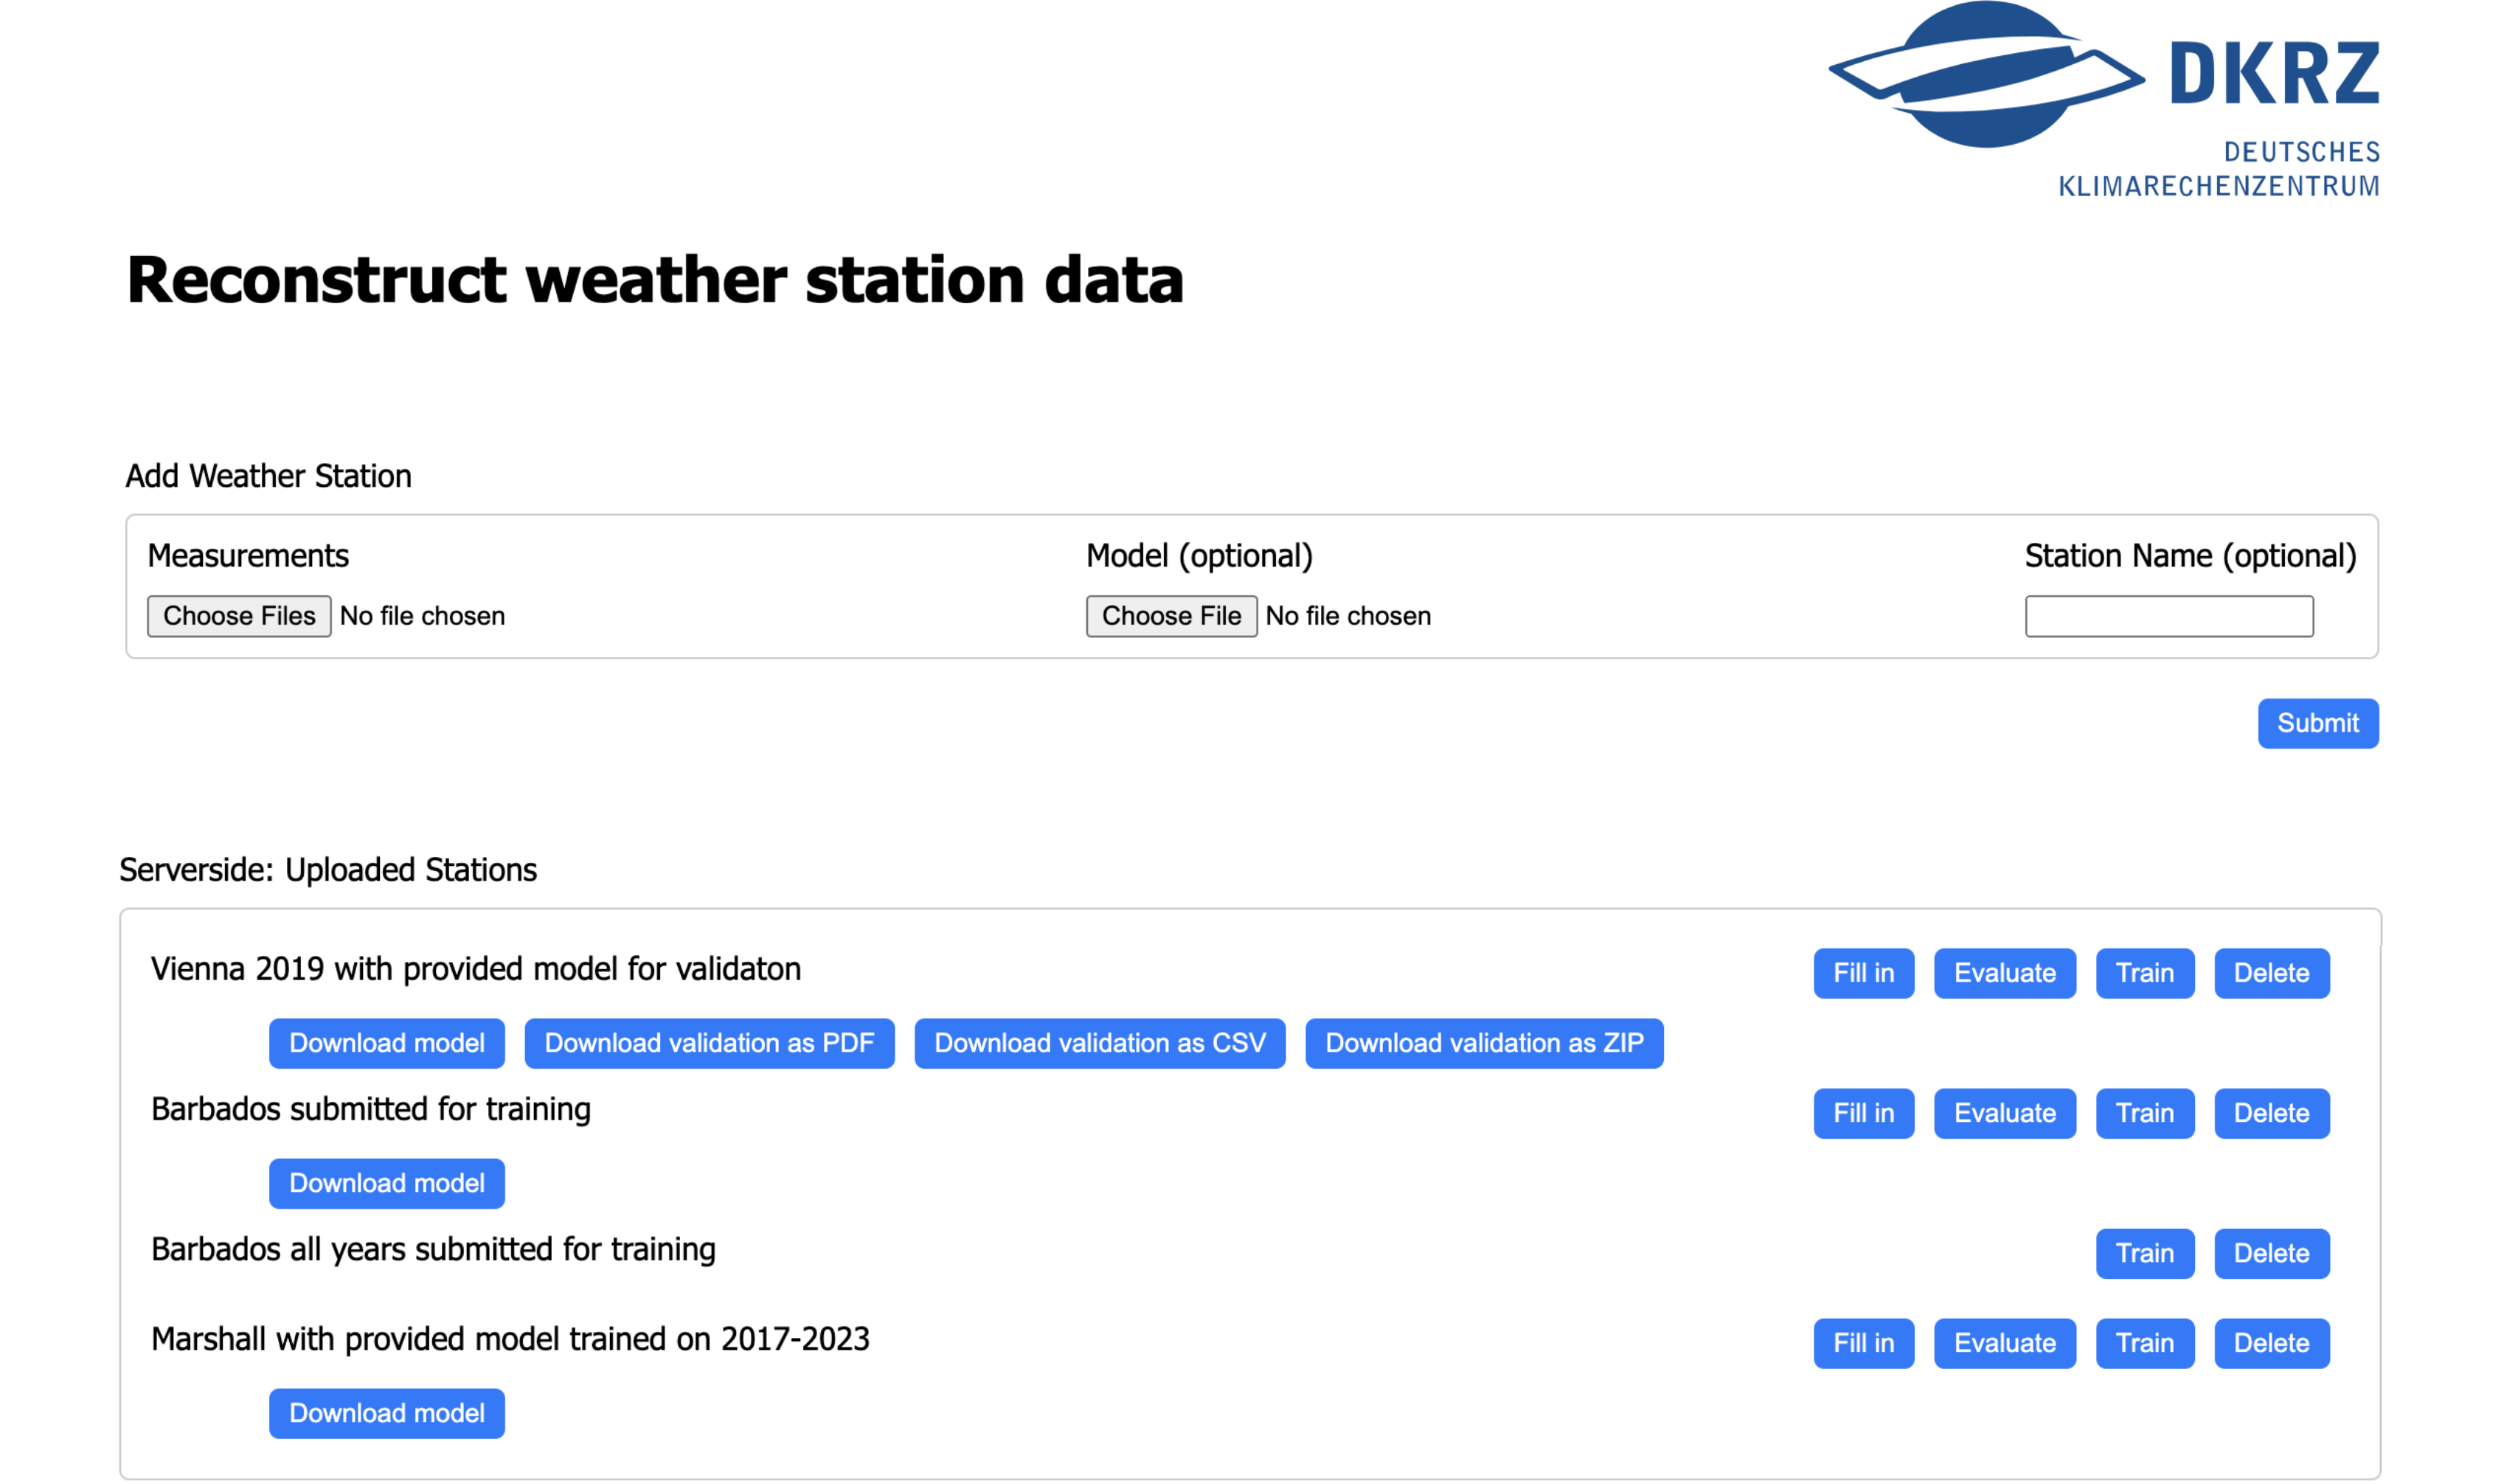
\includegraphics[width=0.5\textwidth]{resources/images/webinterface_screenshot.png}
    \caption{Screenshot of the web interface.}
    \label{fig: webinterface_screenshot}
    \end{wrapfigure}
Additionally, it is possible to monitor the progress of the process through the API.
The details on the API are described in \autoref{sec: api}.
This lays out a sufficient foundation for the implementation of a web interface, which is the main focus of this section.

The interface consists of two areas, one where the user is supposed to submit a "dataset", which in this context is meant as a collection of measurements from a weather station and the station's information such as location, and optionally a custom name and third a trained model for the station that can be provided optionally as well.
If no model is provided the system can train a model and will attach it.

The second area is a list of all datasets that the user has submitted.
The API implementation allows for user identification through a unique token that is passed on to the server when the user submits a dataset, such that the user can then ask to see all datasets owned by them using that same token.
The web interface automatically generates a token for the user and stores it then in the local storage of the browser, such that the user does not have to remember it.

As examples in \autoref{fig: webinterface_screenshot} show each dataset depending on its state has different options available.
The deletion and train buttons all have in common, as no model is necessary to train a model.
Datasets where a model has been provided still could be used to train a new model overwriting the old one.
The \code{Evaluate} and \code{Fill in} buttons to evaluate the model over the timesteps where measurements are available, respectively to evaluate the model over the timesteps where measurements are missing.

Once a process such as training, evaluation, or infilling has been completed for a dataset the user can download the results anytime through the new buttons that appear in the dataset list.
For example, it can be seen in \autoref{fig: webinterface_screenshot} that for the Vienna example, validation has been completed, and the user can now download a PDF with all the plots that compare the predictions with the actual measurements, or a \code{CSV} file with the same data, or a zip file that contains both and the images used in the PDF.
The first Barbados example has a model attached that can be downloaded, meaning either it was provided or generated through training on the server itself.
The second Barbados example has no model attached yet, meaning only the buttons "Train" and "Delete" are available because no model was provided and no training has been done yet.

\subsection{API Endpoints}
\label{sec: api}

As introduced above, the Application Programming Interface (API) is a set of Hypertext Transfer Protocol (HTTP) request messages that define the communication between the web interface and the server.
When a user interacts with the web interface, such as pressing a button, it typically triggers an action on the server or retrieves information. The web interface accomplishes this by sending the appropriate HTTP request to the server. The server processes the request and responds with the necessary information, which is then displayed on the web interface.

Below is a brief description of the available endpoints. The notation \code{<user-token>} and \code{<dataset-id>} are placeholders for the actual user token and dataset ID to identify the correct user or dataset. The user can choose a unique user token for themself; the web interface does that automatically and stores it in the user's browser, while the dataset ID is generated by the server when a dataset is submitted.

\subsubsection*{POST /data-submission}

This endpoint is used to pass a list of measurement files (\code{.dat}) and a metadata file (\code{.rtf}) to the server. Additionally a model file (\code{.pth}) 
Each dataset is associated with a unique ID, and a unique token representing the owner.
The owner's identification token needs to be passed in the request body.
Also, a custom name for the dataset can be passed with the request body.
The dataset ID is created by the server and returned in the response.
The dataset ID is used to refer to the dataset in the following API calls.

\subsubsection*{GET /available-datasets/<user-token>}

For a given user token, this endpoint returns a list of all datasets that the user has submitted.
The user token is passed as a URL parameter.
The response is a list of dictionaries, each containing information about the dataset, such as the dataset ID, the name, and the status of the dataset (e.g. if it is busy training a model and progress percentage).
Moreover, for each dataset, a boolean flag indicates whether a trained model, a validation result or an infilling result is attached. If so, the user can download the results (the last three endpoints).

\subsubsection*{GET /train/<dataset-id>}

A training process is initiated by passing the \code{Station} object of the corresponding data submission to the \code{TrainingExecutor}.
When the training process is finished, the model is saved in the data submission object, and if not timed out yet, the request is answered with the model.
The model is then available through the respective download endpoint.

\subsubsection*{GET /validate-model/<dataset-id>}

Starts the model validation process for the specified dataset.
The process includes downloading ERA5 data for times with available measurements and comparing the model predictions with actual data.
Validation results, including a PDF and CSV file, are saved in the dataset object and can be downloaded using the respective endpoints.

\subsubsection*{GET /fill-in/<dataset-id>}

Initiates the infilling process for the specified dataset.
The process involves using the model to predict missing measurements and generating results that include both the infilled data and related plots.
The infilling results are saved in the dataset object and can be downloaded using the respective endpoint.

\subsubsection*{DELETE /delete-dataset/<dataset-id>}

Deletes the specified dataset from the server along with any associated models, validation results, and infilling results.
The server responds with a confirmation message upon successful deletion.

\subsubsection*{GET /download-model/<dataset-id>}

Allows the requestor to download the trained model associated with the specified dataset.
The server responds by sending the model file as an attachment.

\subsubsection*{GET /download-validation-zip/<dataset-id>}

Allows the requestor to download the validation results as a ZIP file containing both the PDF and CSV files, along with related images.
The server responds by sending the ZIP file as an attachment. There are also endpoints to download the PDF and CSV files exclusively.

\subsubsection*{GET /download-infilling/<dataset-id>}

Allows the requestor to download the infilling results associated with the specified dataset.
The server sends the infilling results file as an attachment if available.